%!TEX root = project.tex

\chapter{System Design}

\section{Unity Environment}

\begin{flushleft}
We aimed to have each player (agent) be capable of observing its own surroundings, so on each frame the agent would be able to make decisions on where it would suit best to move.\par
Each agent needed to be able to calculate distances relative to itself, such as the distance it is from the ball, the distance it is from its own goal, and the distance it is from the opposition goal as seen here in Fig \ref{fig:sd1}.
\end{flushleft}

\begin{figure}[H]
    \centering
    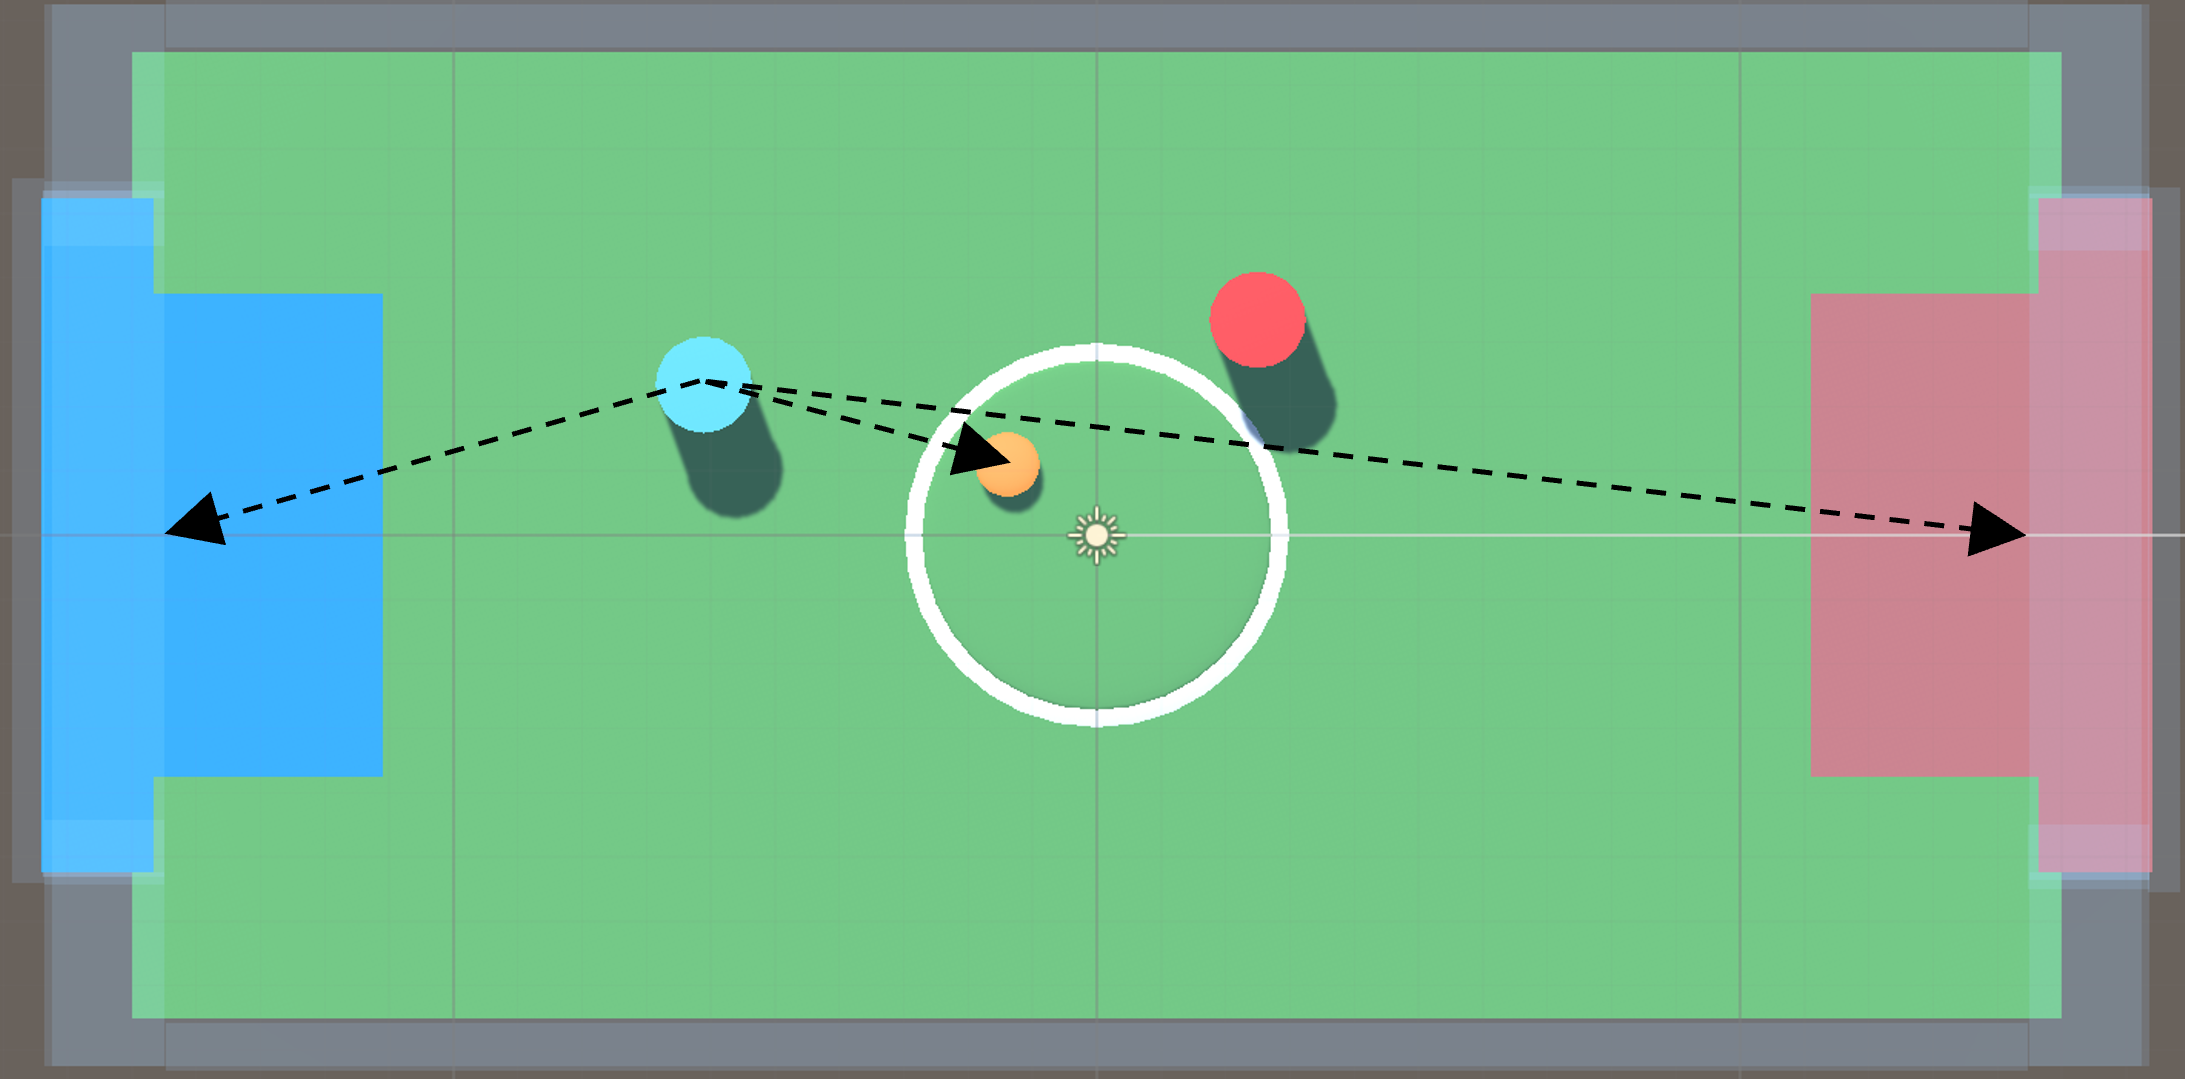
\includegraphics[width=115mm, height=55mm]{img/Image1.png}
    \caption{Distance of blue agent to each goal}
    \label{fig:sd1}
\end{figure}

\begin{flushleft}
Also the agent needed to be able to distancing information relating to the closest opponent to itself, such as the distance the closest opponent is to the ball, the distance the closest opponent is from the opposition goal, and the distance the closest opponent is from the agents own goal as seen here in Fig \ref{fig:sd2}
\end{flushleft}

\begin{figure}[H]
    \centering
    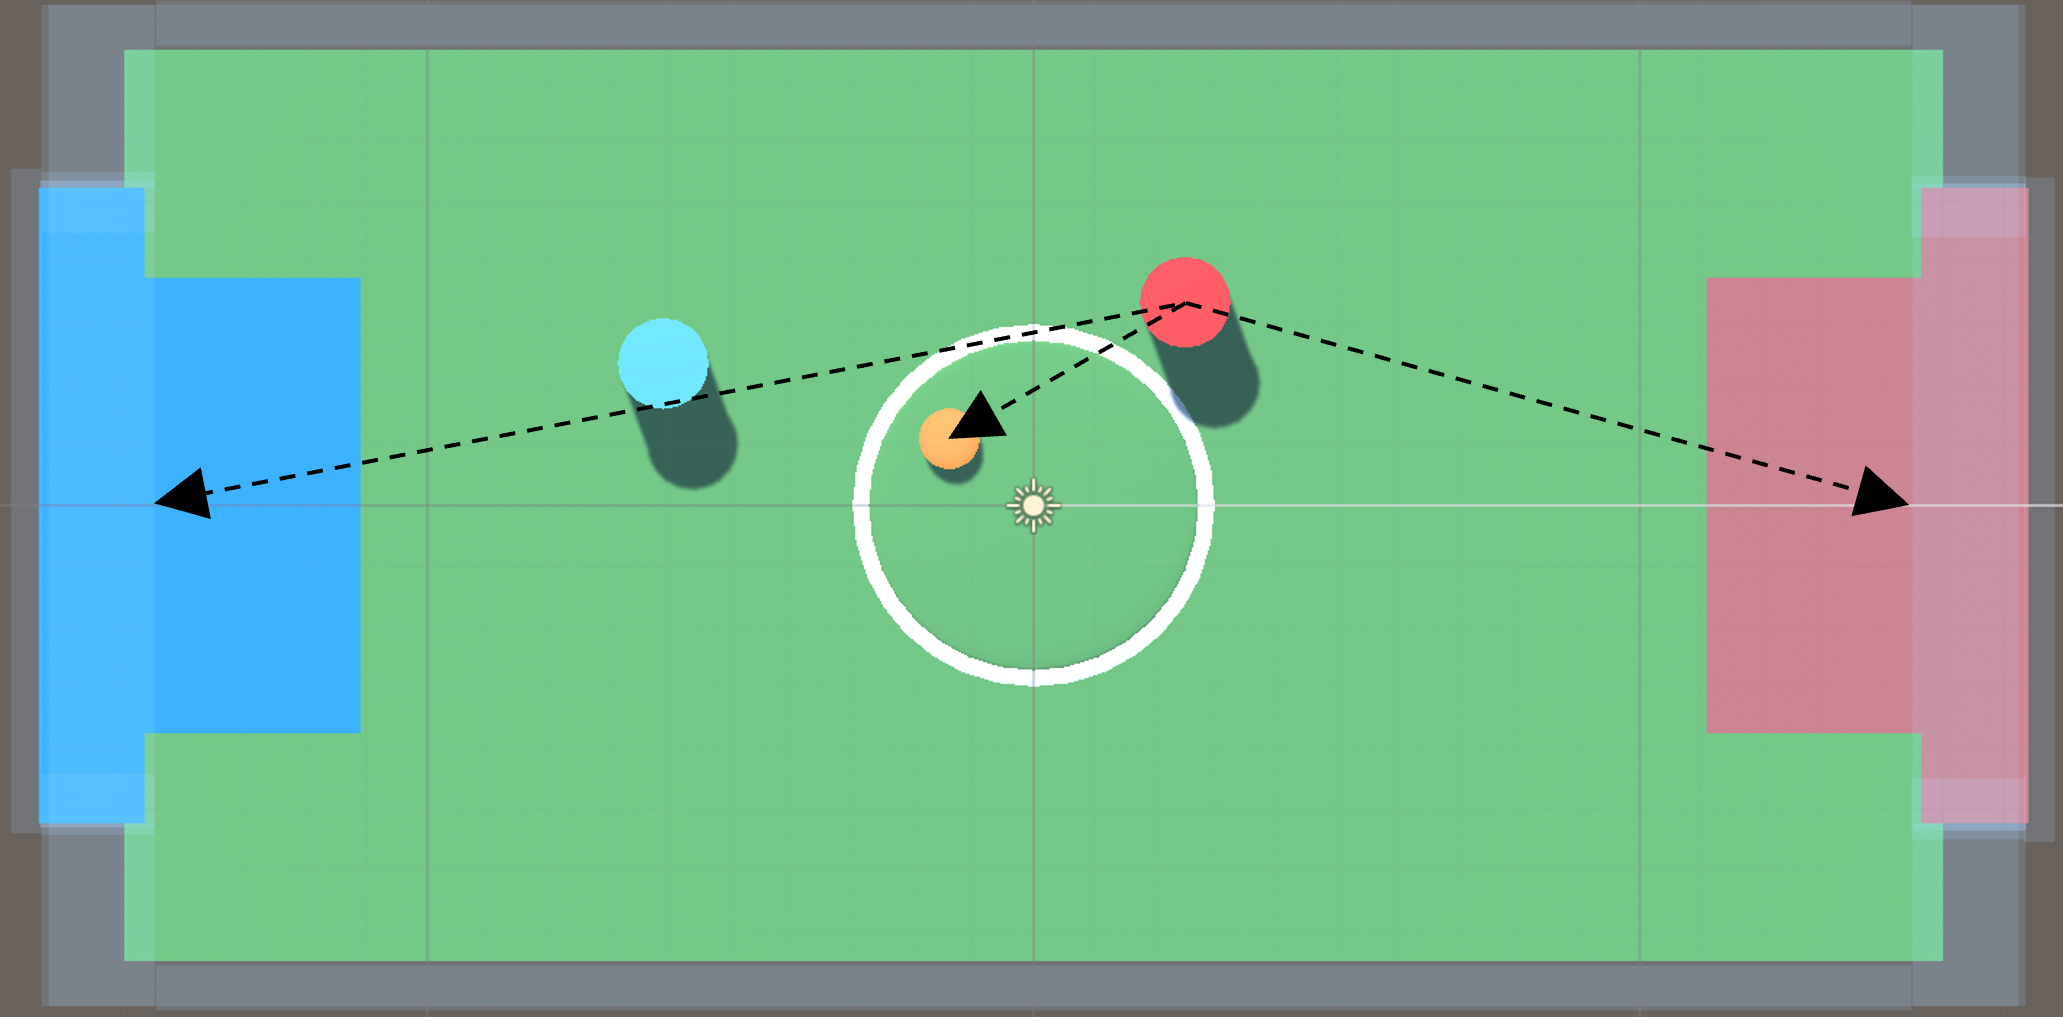
\includegraphics[width=115mm, height=55mm]{img/Image2.png}
    \caption{Distance of red agent to each goal}
    \label{fig:sd2}
\end{figure}

\begin{flushleft}
The overall position of the ball on the pitch would also have to be taken into account, so the agents must have been able to calculate the distance the ball is to the agent's own goal, as well as the distance the ball is to the opposition goal as seen in Fig \ref{fig:sd3}. 
\end{flushleft}

\begin{figure}[h]
    \centering
    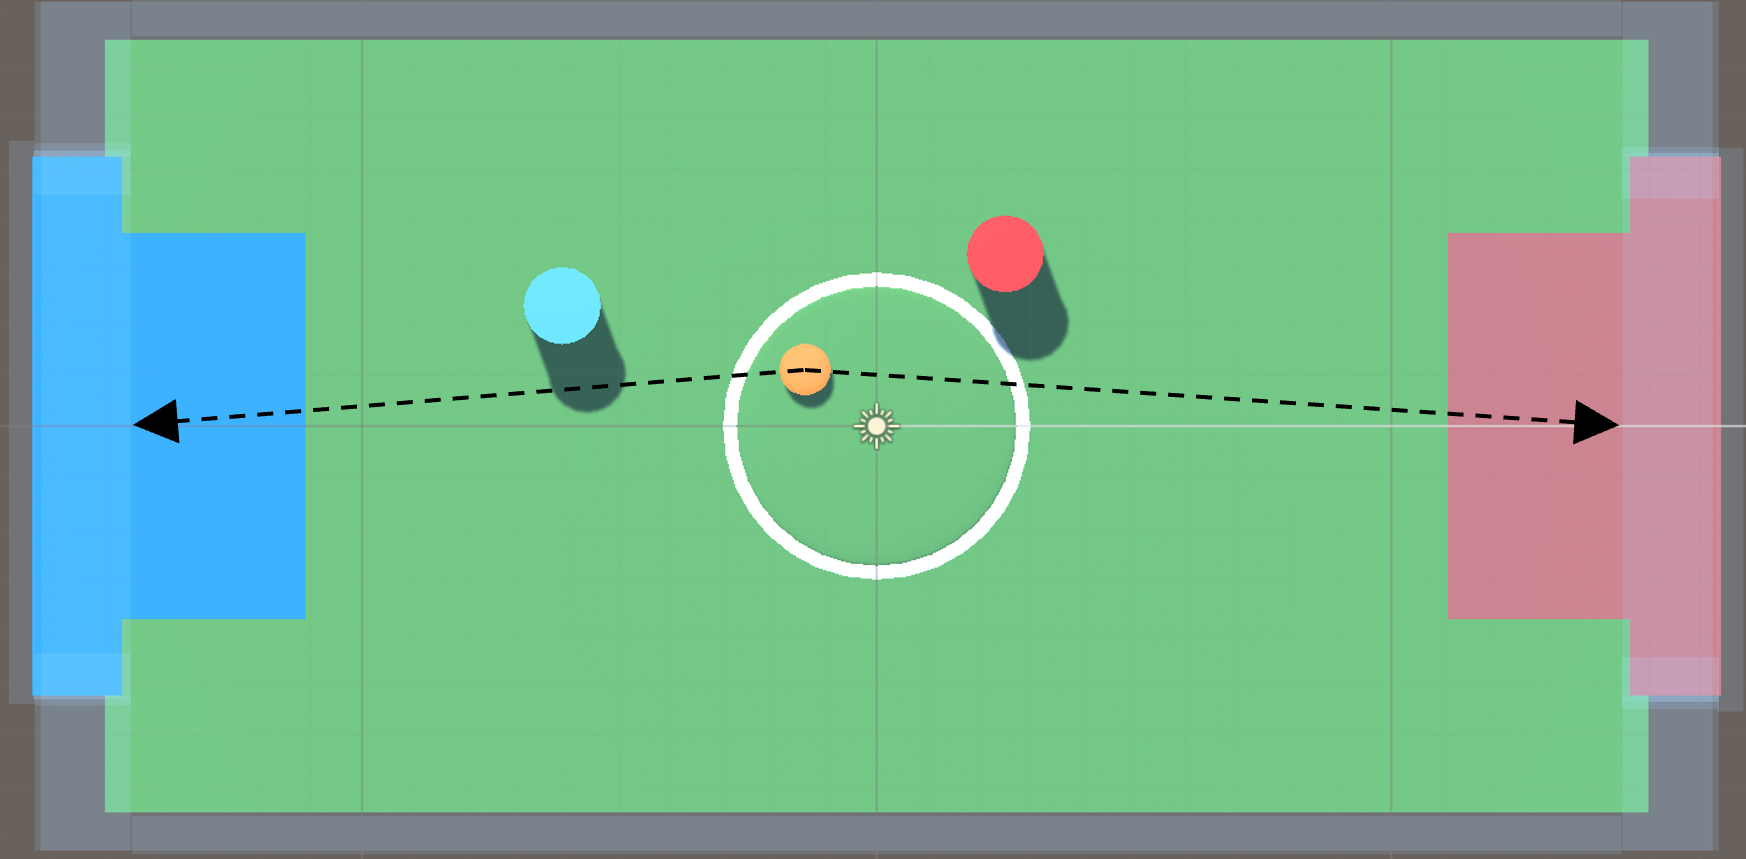
\includegraphics[width=115mm, height=55mm]{img/Image3.png}
    \caption{Distance of ball to each goal}
    \label{fig:sd3}
\end{figure}

\begin{flushleft}
Each agent needed to know what type of player they were, be it a goalkeeper, defender, or striker, and adjust its decision making accordingly, for example, in some scenarios it would be better for a goalkeeper to stay protecting the goals instead of rushing out to challenge the opponent with the ball, however a defender or striker might decide to push forward and challenge the ball in the same scenario, be it there is a goalkeeper positioned in their goals.

Along with each agent knowing which type of player they are, they also need to be able to detect what type of player the closest opposition is, as this could also affect the decision the agent makes, whether the agent should attempt to challenge the ball or if they are better off positioning themselves elsewhere.

Finally, the agent needs to be able to determine the angle the ball sits between themselves and the opposition goals, as well as the angle the ball sits between the agent and their own goal as seen in Fig \ref{fig:sd4}. These angles need to be considered as they will also influence the agent’s decision when moving frame by frame.
\end{flushleft}

\begin{figure}[H]
    \centering
    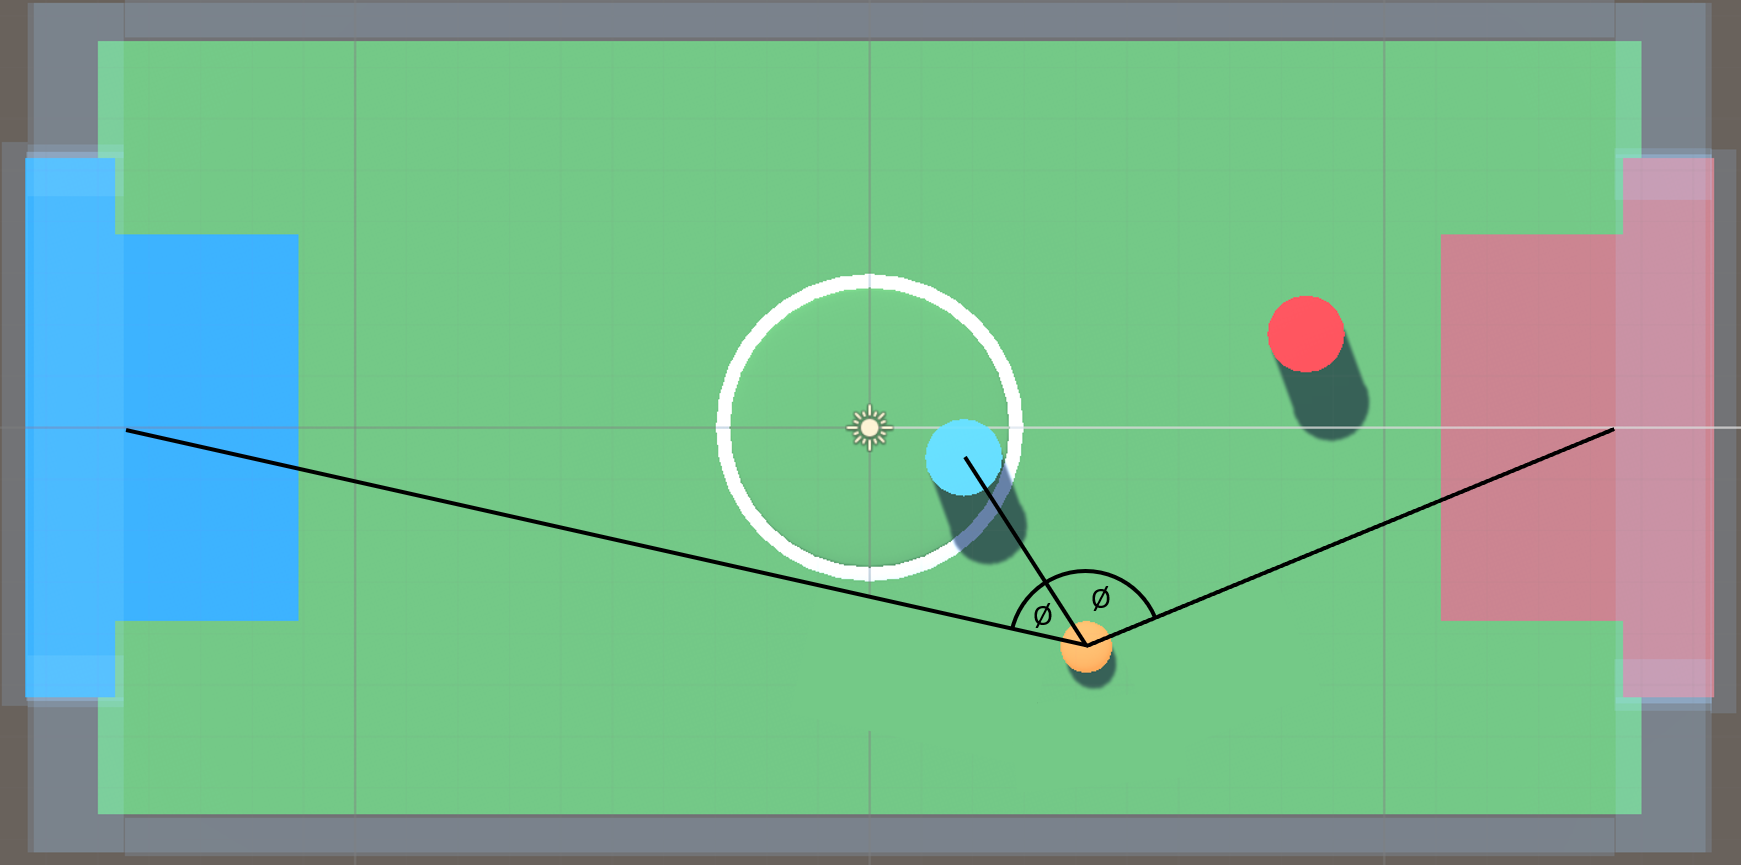
\includegraphics[width=115mm, height=55mm]{img/Image5.png}
    \caption{Angle of ball to goals and player}
    \label{fig:sd4}
\end{figure}

\begin{flushleft}
For example, it would be better for the goalkeeper to position themselves between the ball and the goal here, instead of simply rushing towards the ball and attempting to challenge the opponent as displayed in Fig \ref{fig:sd5}.
\end{flushleft}

\begin{figure}[H]
    \centering
    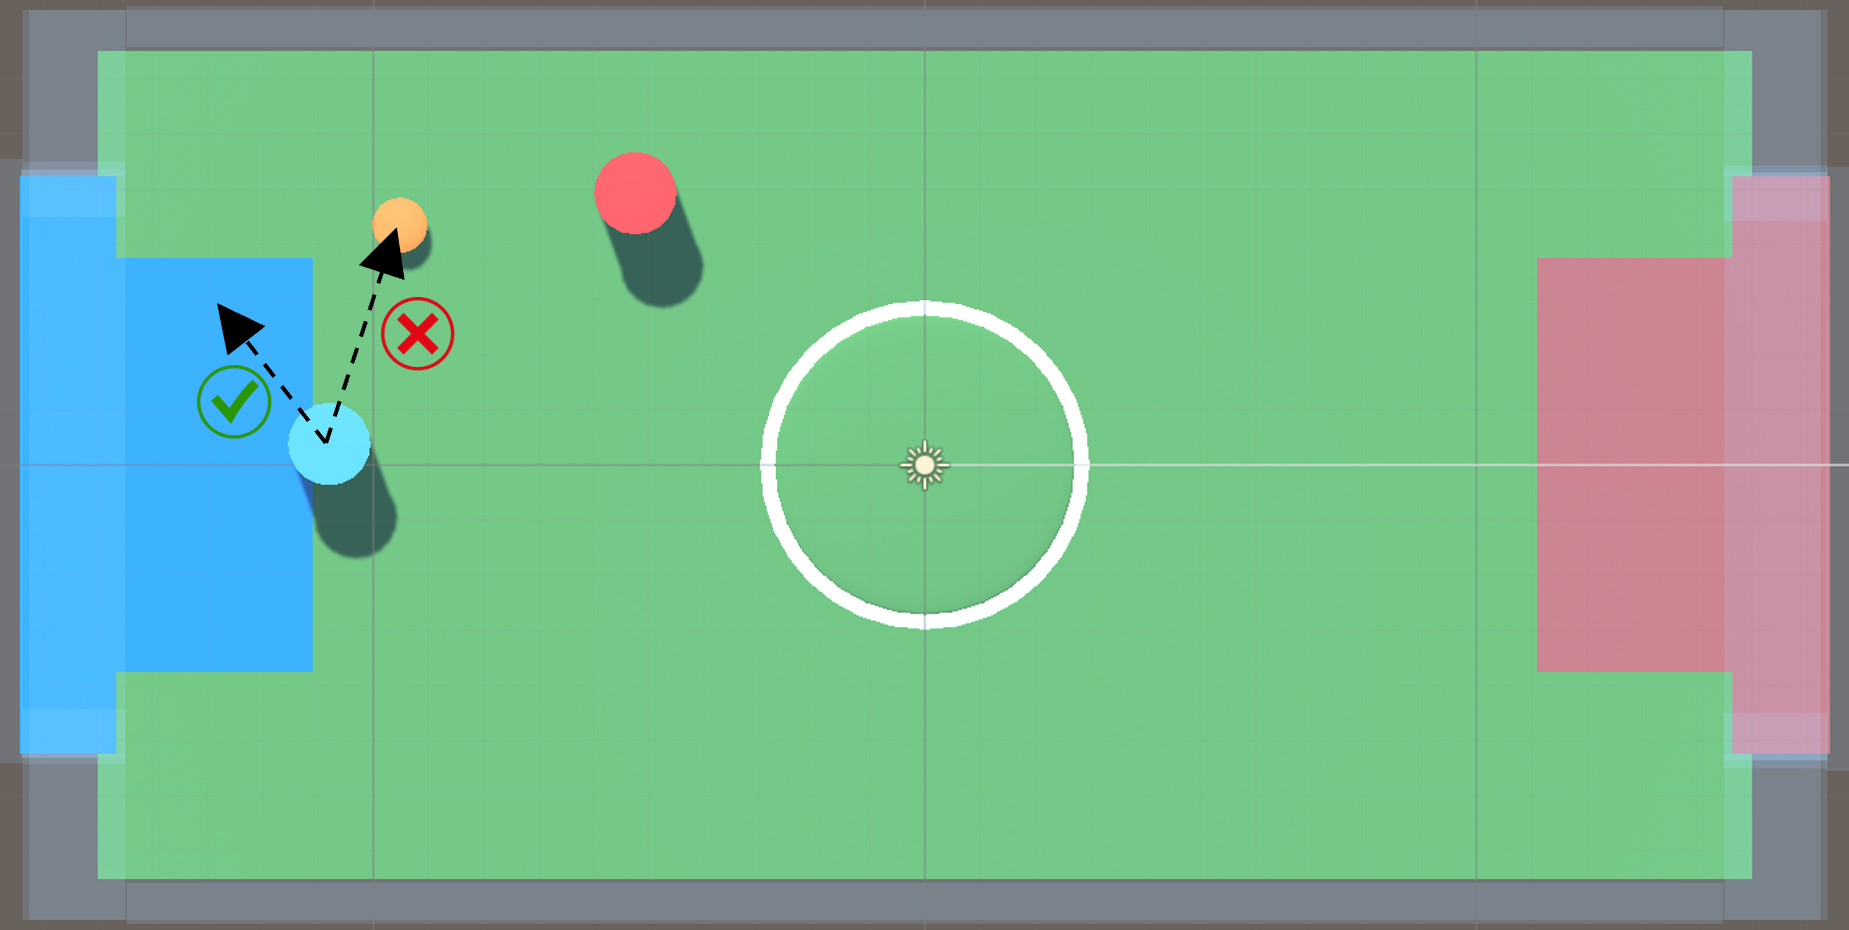
\includegraphics[width=115mm, height=55mm]{img/Image4.png}
    \caption{Ball prioritizing stopping goal over chasing ball}
    \label{fig:sd5}
\end{figure}

In the “Soccer-Rand-Enviro” scene, a single agent is placed on the field. This scene is ment to offer a clear view of the random inputs notebook at work, leaving the entire area free for the agent to spawn into on each epoch run of the notebook. The scene originated as the starting scene we aimed to use to train the first agent in, and once we had a single agent working as we intended, we could move onto other scenes with more agents.

In the “Soccer” scene, 6 agents are positioned on the field. This scene was ment to be the next step after getting a single agent working as intended. We were going to have multiple agents working with each other, and logically playing with teammates to attempt to score. Currently this scene acts as a showcase of what we wanted the project to perform like, with agents keeping there own positions on the pitch and attempting to score in the opositions goals.

In the “Soccer-2” scene, more agents have been added to the pitch, making the total add up to 14 agents. This scene was going to offer us an environment to fully test the capabilities of our trained agents, allowing them to have multiple more teamates to incorporate into the input data and expand there complexity. Unfortunity we never got to use this scene as we wanted, and rather only ran the random input notebook with it, since we couldn’t pass the nessessary input data back to the network.

\section{Jupyter Notebook}

Neural Network
The design for the neural network architecture consisted of 14 input nodes, a single hidden layer of 16 nodes, and 8 output nodes. The input nodes consist of multiple different value taken from the environment, including factors such as the type of agent being controlled, distances between the different agents on the pitch and the ball, the overall position of the ball on the pitch, as well as data pertaining to the angle the ball is between the agent and the target goals. The output nodes consist of each direction the agent could move at each episode. Meaning the neural network will use the data taken from the current state of the environment and the agent will move in the direction that it believes will end with the best outcome.

As many pages as needed.
\begin{itemize}
\item Architecture, UML etc. An overview of the different components of the system. Diagrams etc… Screen shots etc.
\end{itemize}

%\begin{table}[h]
%  \centering
%  \begin{tabular}{x{2cm}p{3cm}}
%    \toprule \\
%    Column 1 & Column 2 \\
%    \midrule \\
%    Rows 2.1 & Row 2.2 \\
%    \bottomrule
%  \end{tabular}
%  \caption{A table.}
%  \label{table:mytable}
%\end{table}